% Generated from ICA_2.docx — re-run: python scripts/ica2_emit_latex.py
\chapter{System Design}
\label{ch:design}

\section{Introduction}

This chapter presents the architectural and detailed design of the proposed IoT security monitoring application. The design translates the functional and non-functional requirements defined in Chapter 8 into a coherent system structure that supports security-driven availability monitoring and anomaly detection. Emphasis is placed on modularity, scalability, and usability to ensure suitability for home and small-to-medium business (SMB) environments.

\section{Overall System Architecture}

The system adopts a client--server architecture consisting of three primary layers: a user-facing frontend, a backend application layer, and a persistent data storage layer. This separation of concerns supports maintainability and scalability while enabling independent evolution of system components.

At a high level, users interact with the platform through a web-based dashboard. The frontend communicates with the backend via secure API endpoints, allowing users to register devices, view status information, and receive alerts. The backend is responsible for authentication, device management, heartbeat processing, anomaly detection, and alert generation. Persistent storage is used to retain user data, device metadata, and historical monitoring records.

\begin{figure}[htbp]
  \centering
  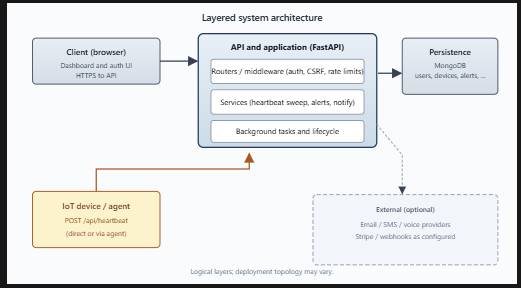
\includegraphics[width=0.92\textwidth]{figures/ICA2_embed_5.png}
  \caption{System Architecture}
  \label{fig:ica2_5}
\end{figure}

\section{Frontend Design}

The frontend is designed to prioritise clarity and ease of use for non-expert users. A dashboard-centric interface provides a consolidated view of all registered devices, their current availability status, and recent alerts. Visual indicators are used to distinguish between normal operation and abnormal conditions, reducing cognitive load for users.

Core frontend components include:

A login and authentication interface to ensure secure access.

A device management view allowing users to add, edit, or remove registered devices.

A monitoring dashboard presenting real-time status and historical trends.

An alert view highlighting active and resolved incidents.

The frontend design deliberately avoids excessive configuration options, reflecting the requirement for usability and accessibility. Instead, sensible defaults are applied to monitoring thresholds, with limited customisation available for advanced users.

\begin{figure}[htbp]
  \centering
  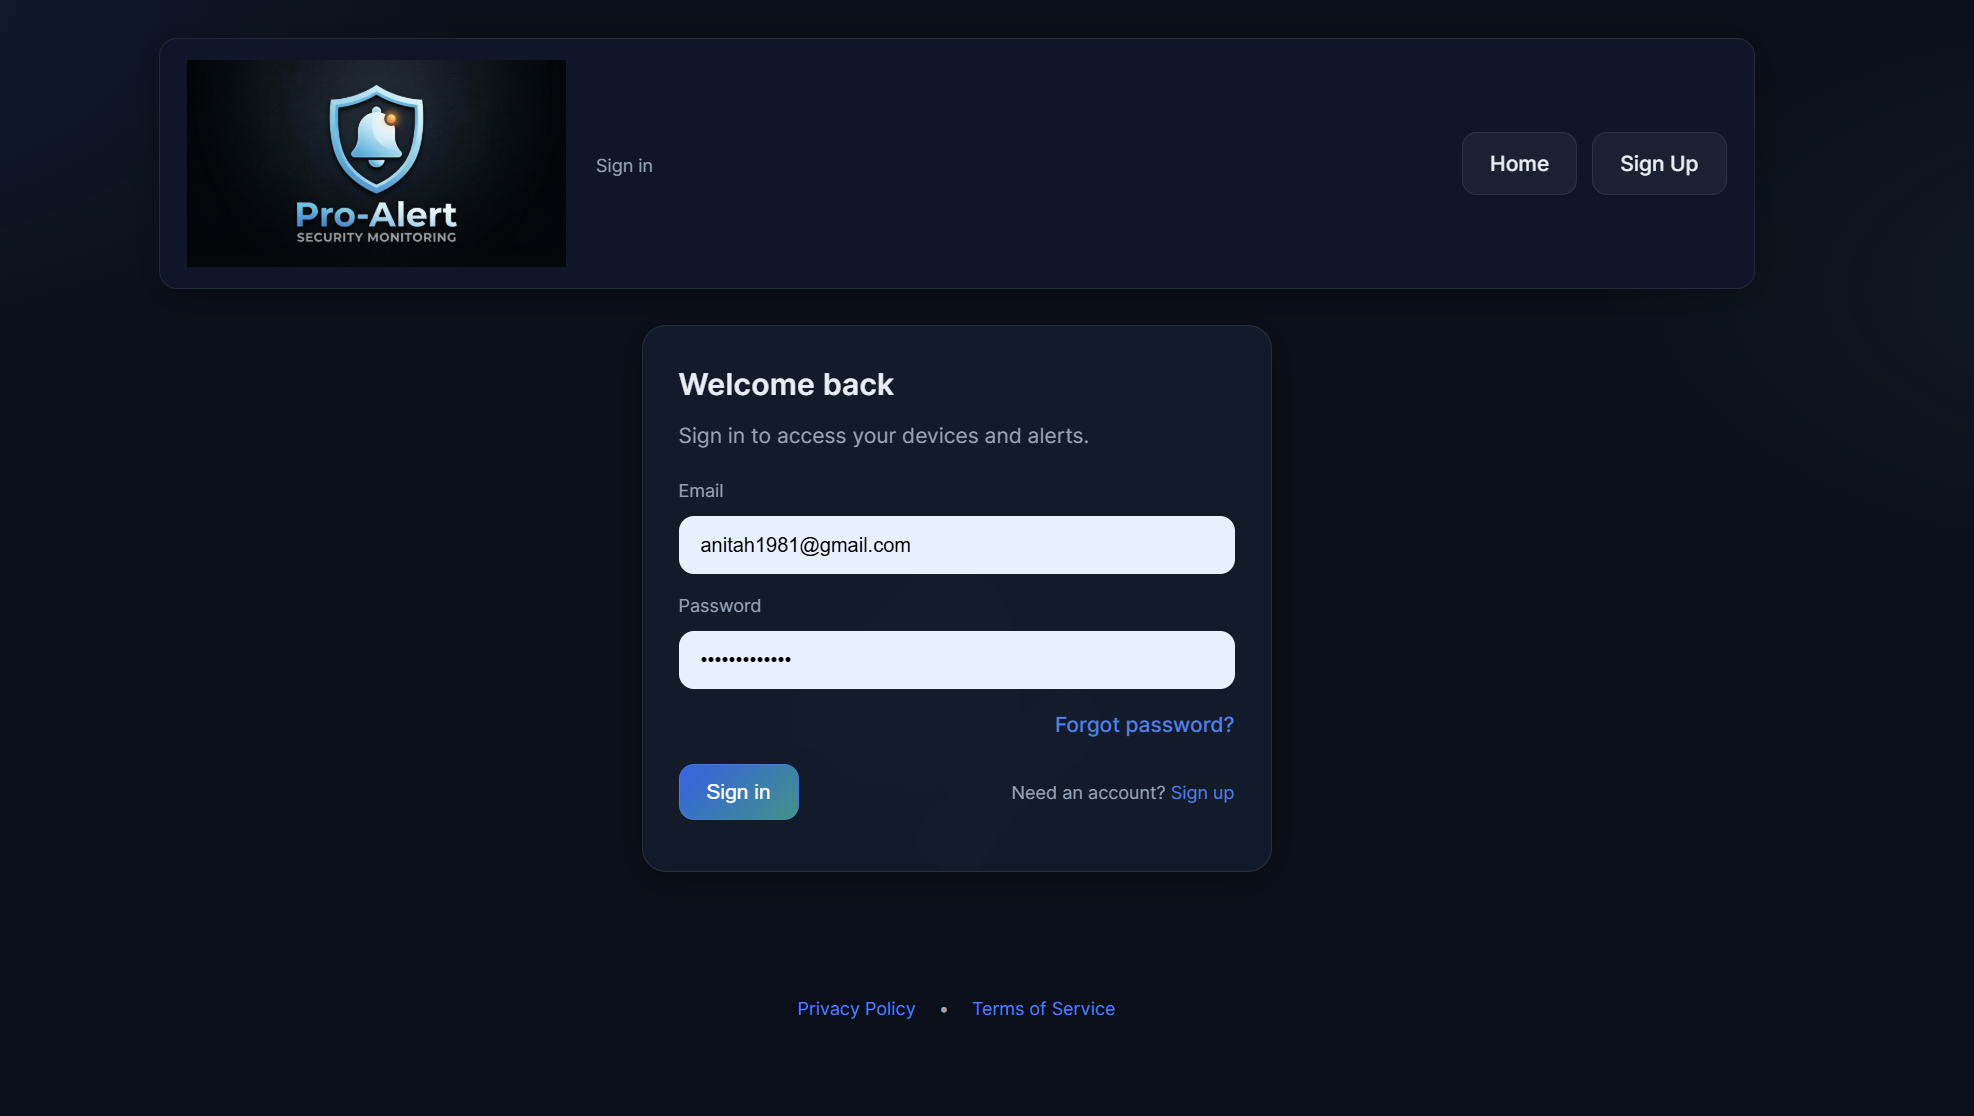
\includegraphics[width=0.92\textwidth]{figures/ICA2_embed_6.png}
  \caption{Login and Authentication Interface}
  \label{fig:ica2_6}
\end{figure}

\begin{figure}[htbp]
  \centering
  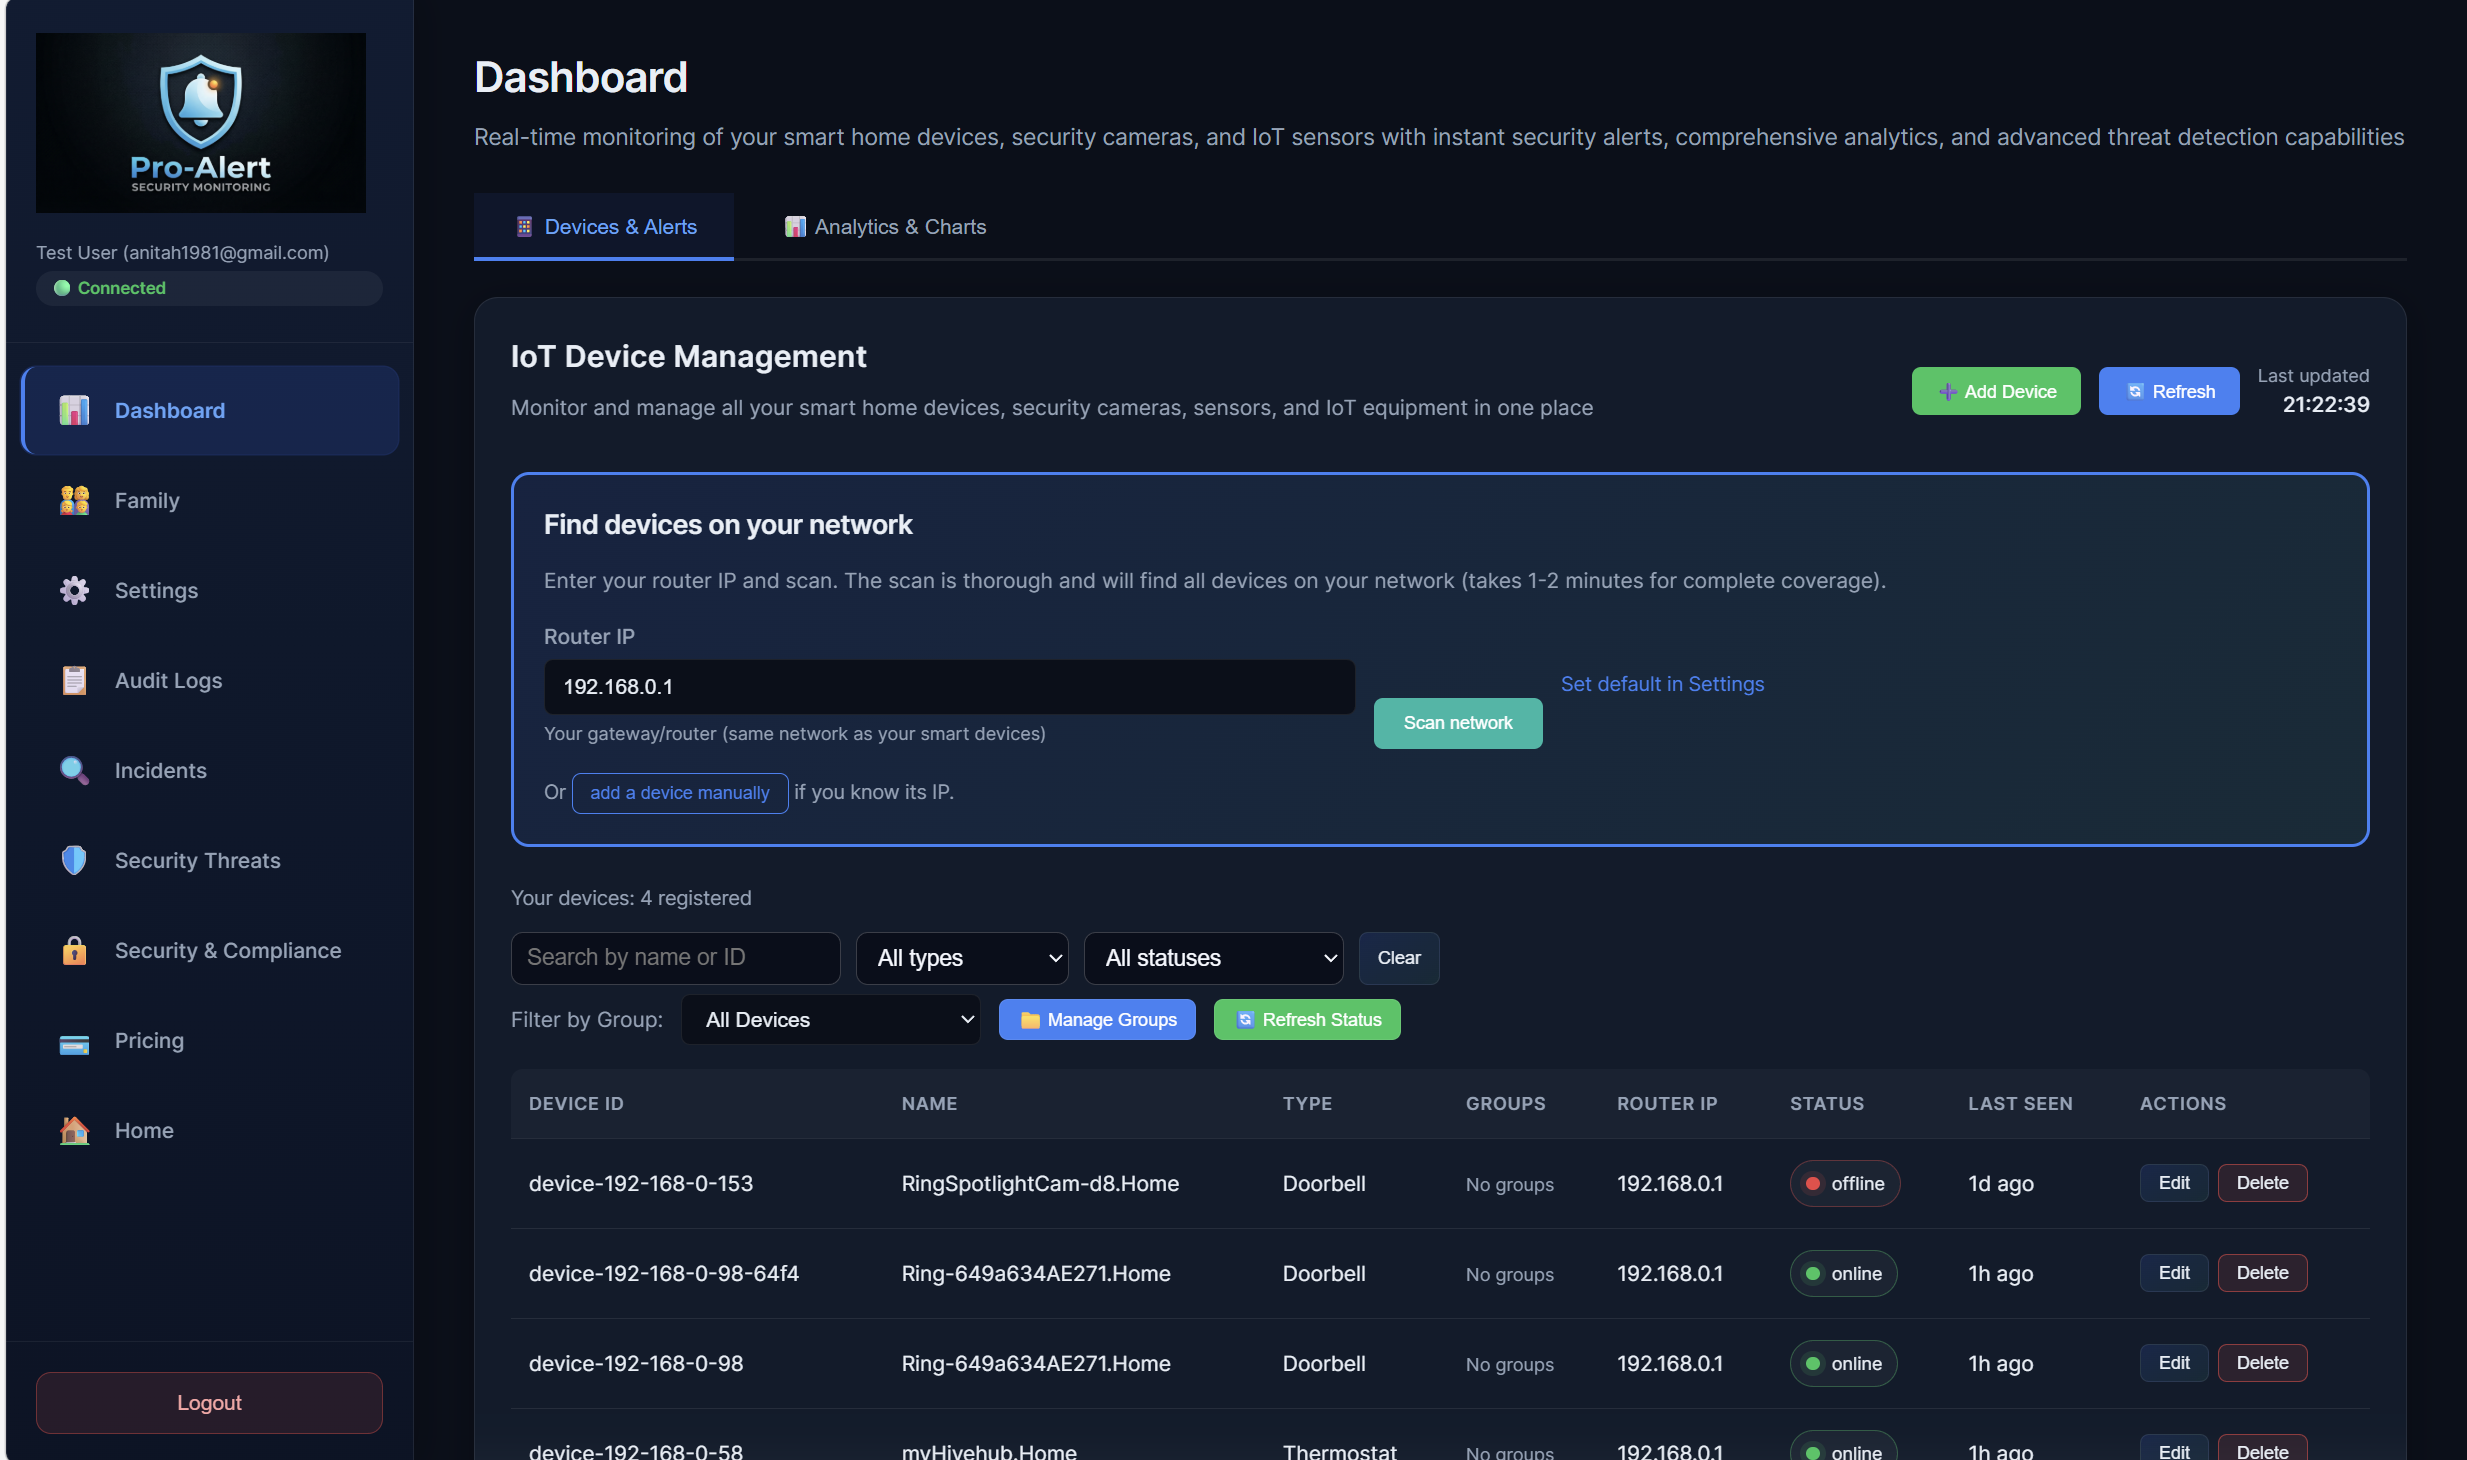
\includegraphics[width=0.92\textwidth]{figures/ICA2_embed_7.png}
  \caption{Dashboard}
  \label{fig:ica2_7}
\end{figure}

\begin{figure}[htbp]
  \centering
  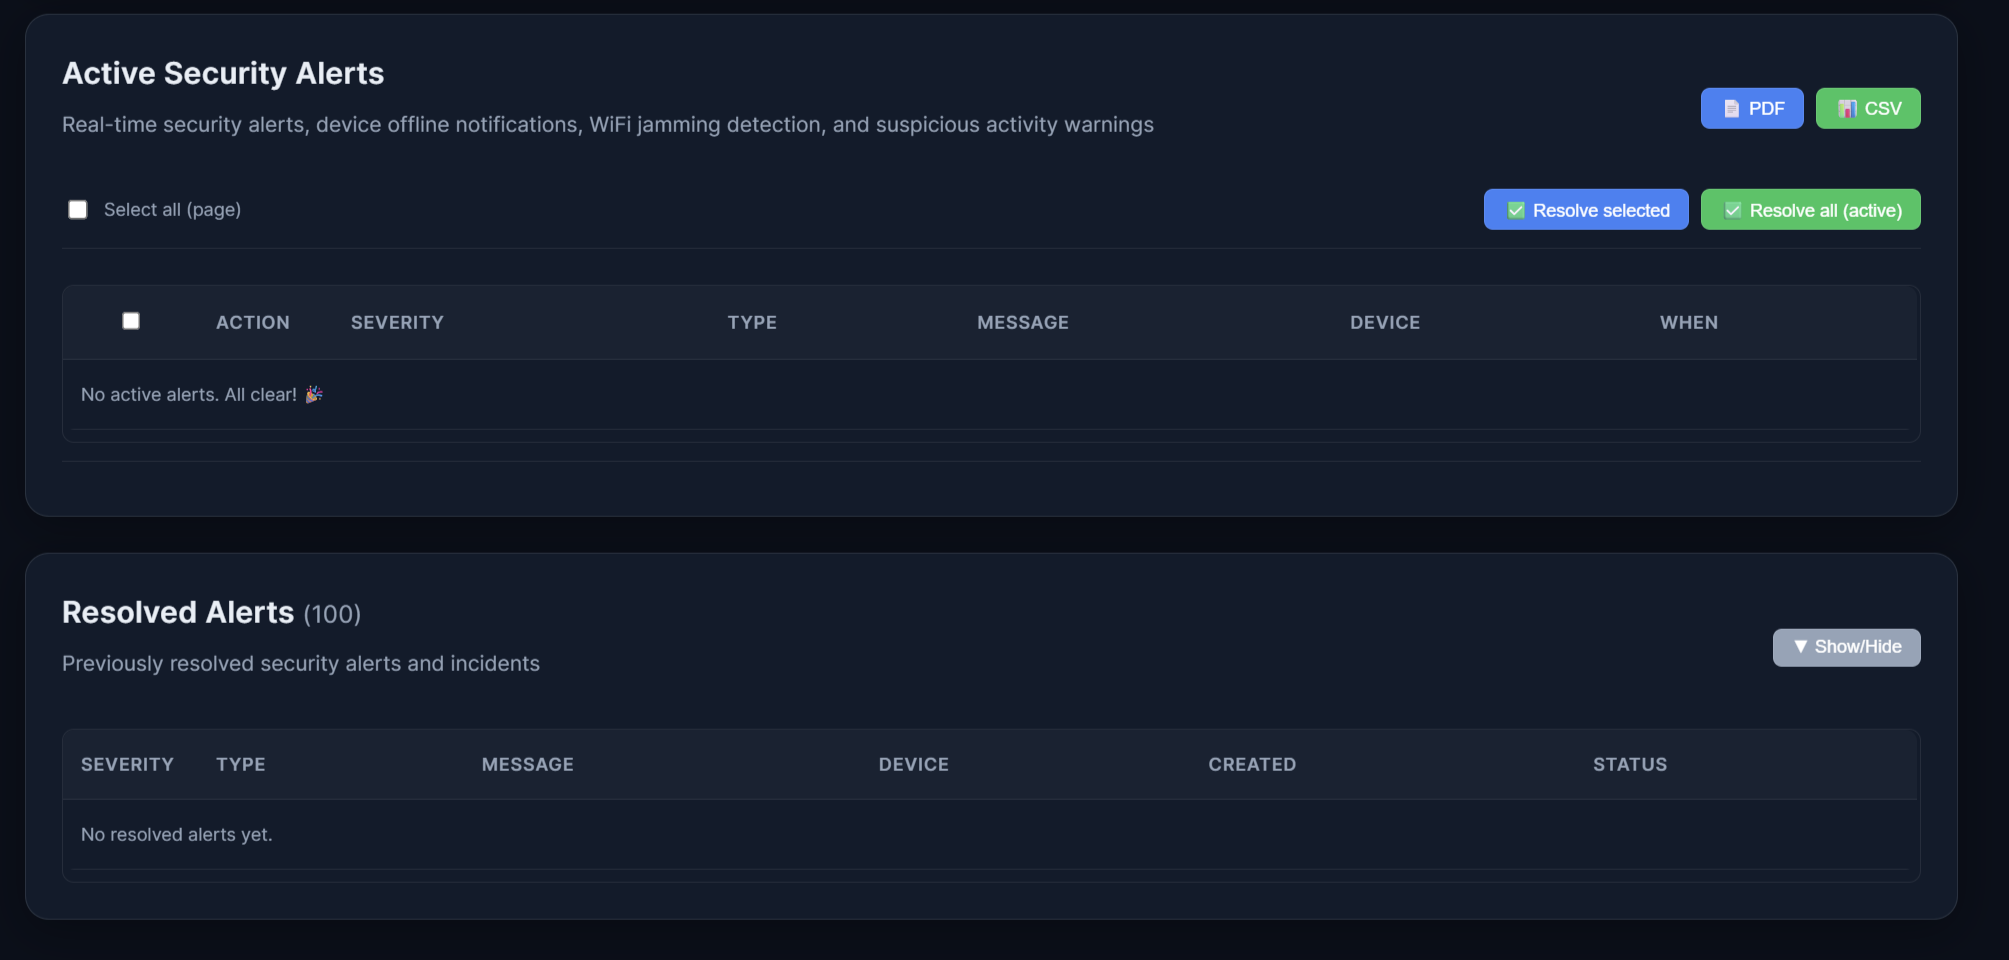
\includegraphics[width=0.92\textwidth]{figures/ICA2_embed_8.png}
  \caption{Active and Resolved Alerts}
  \label{fig:ica2_8}
\end{figure}

\section{Backend Design}

The backend serves as the central control point for system logic and security enforcement. It exposes a set of API endpoints that facilitate communication between the frontend and backend services. Authentication and authorisation mechanisms ensure that users can only access their own device data.

Key backend responsibilities include:

Managing user accounts and authentication sessions.

Handling device registration and maintaining unique device identifiers.

Receiving and processing heartbeat signals.

Detecting availability failures and anomalous behaviour.

Generating and dispatching alerts.

The backend is implemented using a modular design approach, with distinct services or modules responsible for specific functionality. This modularity supports maintainability and aligns with the non-functional requirement for future extensibility.

\section{Heartbeat Monitoring Mechanism}

Heartbeat monitoring is a core design feature of the system and underpins availability detection. Each registered device is expected to report its presence at regular intervals, either directly or via an intermediary process. The backend records the timestamp of each received heartbeat and compares it against expected intervals.

If a heartbeat is not received within a predefined tolerance window, the system flags the device as potentially unavailable. This approach enables detection of both accidental disconnections and deliberate interference, such as Wi-Fi jamming (TechHive, 2024). The tolerance window is designed to balance responsiveness with resilience to transient network issues, reducing the likelihood of false positives.

Where configured, heartbeats may also be accepted via a \emph{device agent} key, so a lightweight on-device or edge client can report liveness without holding full user credentials---useful on less trusted networks. This path is optional and secondary to the direct authenticated API flow emphasised in testing.

Heartbeat data is logged persistently to support historical analysis and evaluation.

\begin{figure}[htbp]
  \centering
  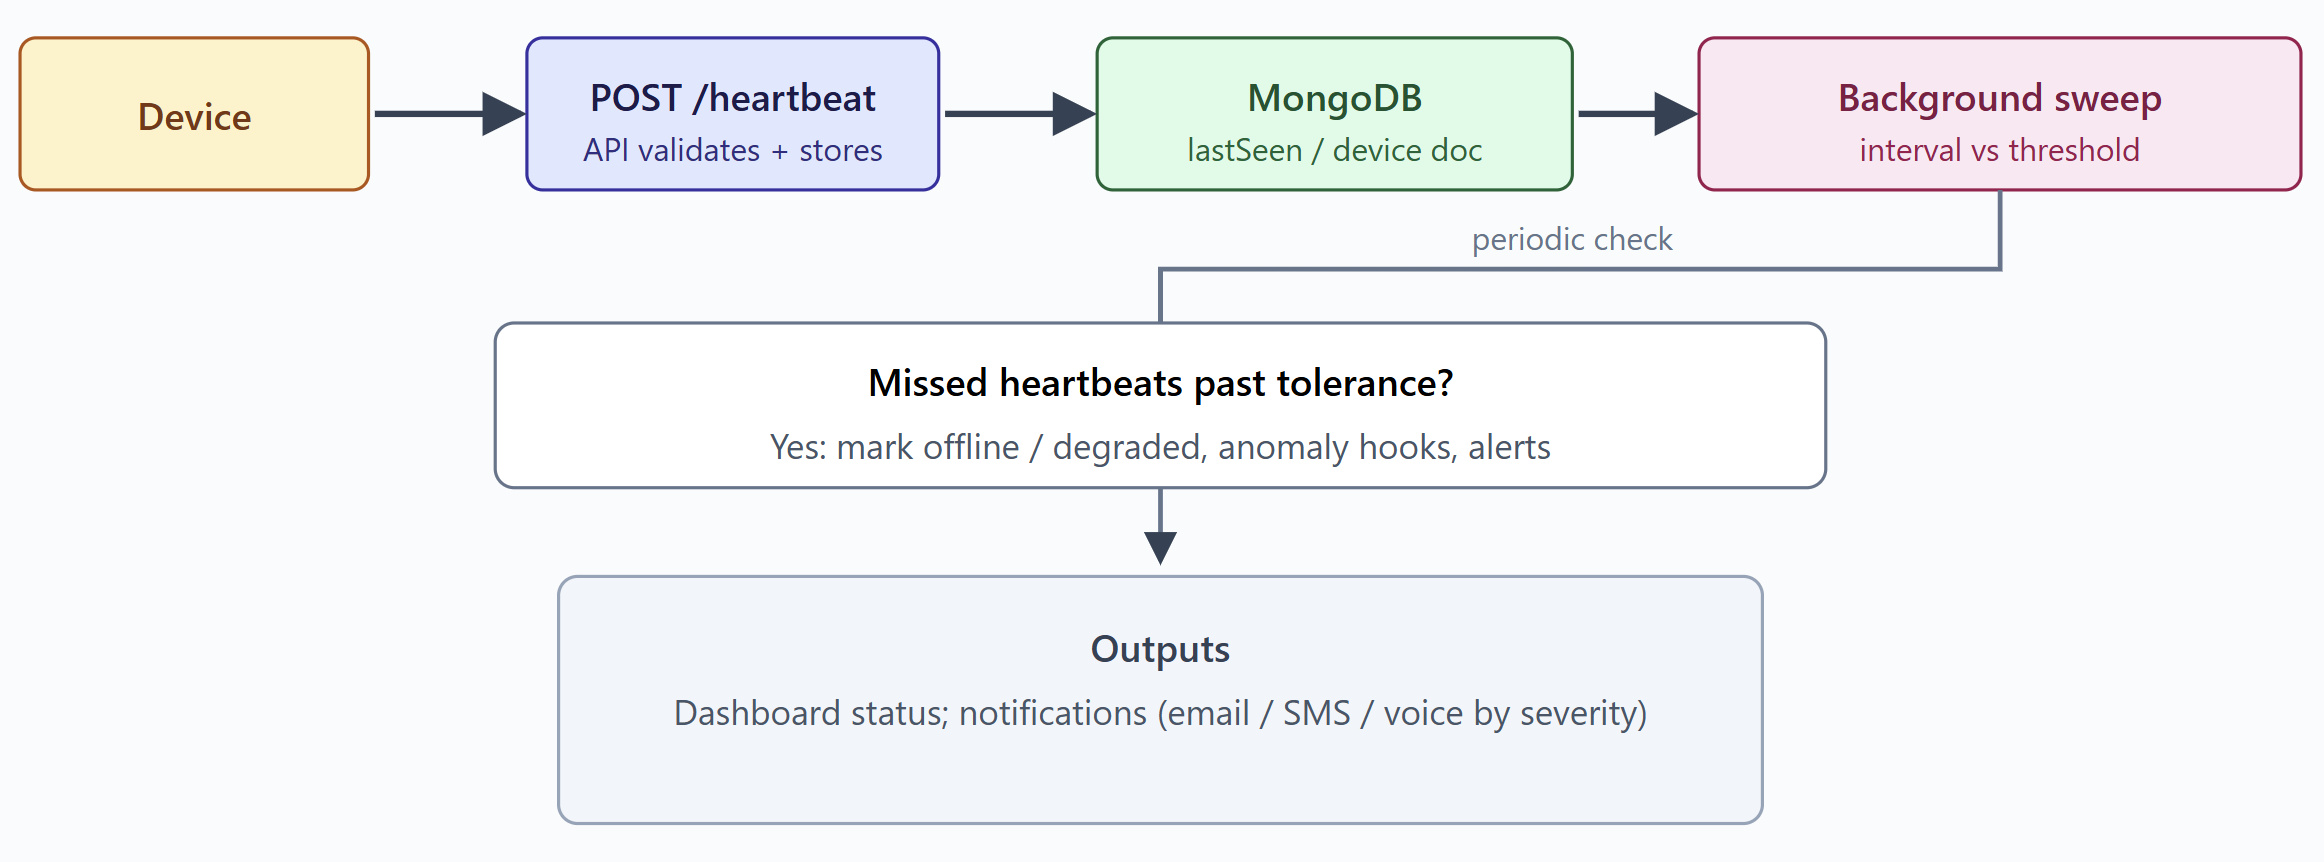
\includegraphics[width=0.92\textwidth]{figures/ICA2_embed_9.png}
  \caption{Heartbeat Mechanism}
  \label{fig:ica2_9}
\end{figure}

\section{Anomaly Detection Logic}

Anomaly detection within the system is implemented using a behaviour-based approach rather than deep packet inspection. This design choice reflects both resource constraints and privacy considerations, as traditional deep packet inspection is often too heavy and invasive for consumer IoT hardware (Ahmad \& Shah, 2024). The system analyses deviations from expected device behaviour, including irregular heartbeat intervals, repeated disconnections, and sudden status changes.

Multiple indicators are considered when evaluating anomalies, allowing the system to correlate events and improve detection accuracy. For example, a single missed heartbeat may not trigger an alert, whereas repeated missed heartbeats combined with connectivity changes may indicate a more serious issue. This rule- and heuristic-based approach provides transparency and interpretability, enabling users to understand why alerts are generated. It also aligns with the project's emphasis on accessibility and practical deployment.

At implementation level, supplementary modules support the same philosophy without introducing opaque machine-learning stacks: for example, IP-change and pattern checks in a dedicated security monitor, and time-window grouping of related alerts into \emph{incidents} for clearer dashboard review. These remain heuristic and explainable, consistent with the design above.

\section{Alerting and Notification Design}

Alerting is designed to provide timely and actionable information without overwhelming users and risking alert fatigue---a well-documented issue that can lead to users ignoring critical security warnings (Hassan et al., 2020). When availability failures or anomalies are detected, alerts are generated and displayed prominently within the dashboard.

Alerts include contextual information such as device identity, time of occurrence, and the nature of the detected issue. Where feasible, alerts may also be delivered through supplementary notification channels to ensure visibility even when users are not actively monitoring the dashboard. The system supports alert acknowledgement and resolution tracking, enabling users to distinguish between active issues and historical events.

\section{Data Storage and Management}

Persistent storage is used to retain user accounts, device metadata, heartbeat records, and alert logs. Data models are designed to support efficient querying and historical analysis while adhering to data minimisation principles (ICO, 2024). Sensitive information is stored securely, and access controls are enforced at the application level.

Historical data supports both user-facing features, such as trend visualisation, and evaluation activities described in later chapters. Data retention policies are designed to balance analytical value with privacy considerations.

\begin{figure}[htbp]
  \centering
  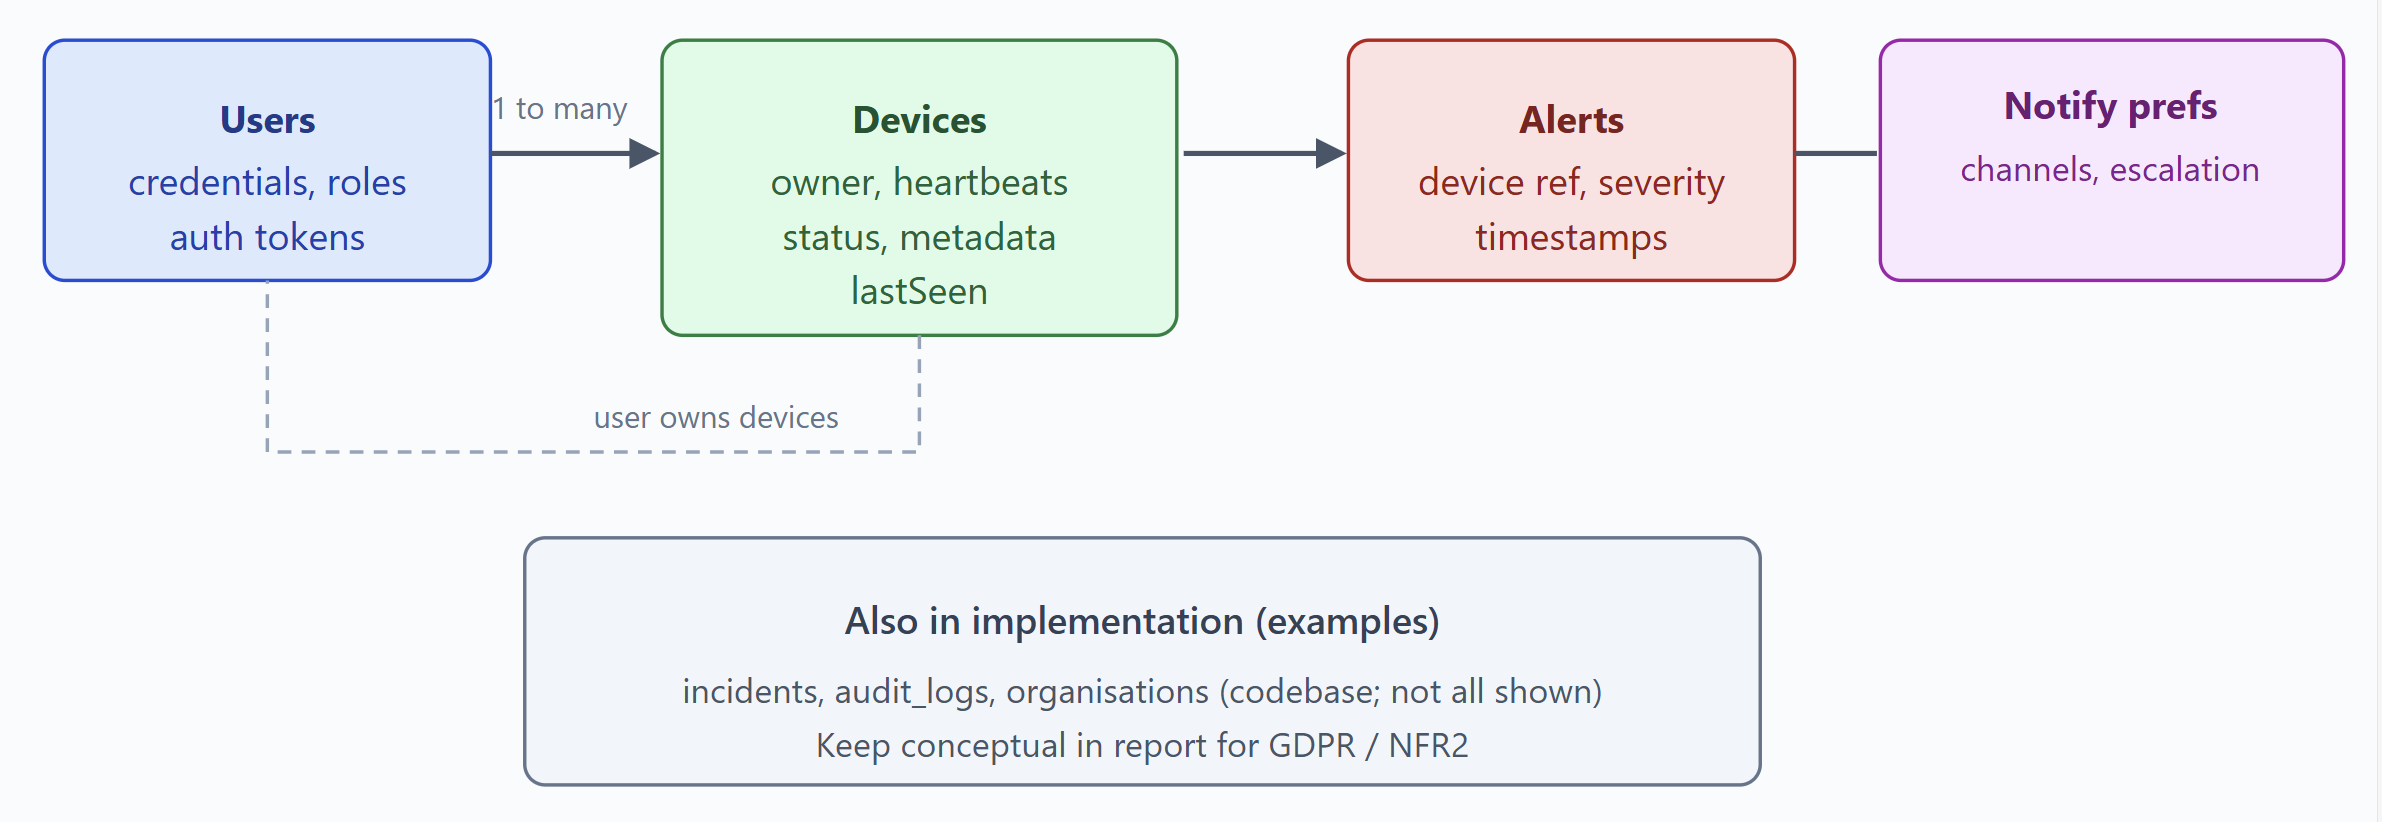
\includegraphics[width=0.92\textwidth]{figures/ICA2_embed_10.png}
  \caption{Data Storage}
  \label{fig:ica2_10}
\end{figure}

\section{Design Justification and Trade-offs}

Several design trade-offs were made to align the system with project constraints and objectives. The decision to avoid deep packet inspection reduces detection granularity but improves deployability and privacy compliance. Similarly, the use of heuristic-based anomaly detection prioritises transparency and simplicity over advanced machine learning techniques.

These trade-offs are justified by the target deployment context. For home and SMB users, timely awareness of availability and abnormal behaviour provides significant security value without the complexity of enterprise-grade solutions.

\section{Summary}

This chapter has detailed the system design and architectural decisions underpinning the proposed IoT security monitoring application. By mapping requirements to concrete design elements, the chapter demonstrates a structured and intentional approach to system development.
